% created on 30/03/2020
% @author : ebazan
\phantomsection
\chapter*{Introduction}
\addcontentsline{toc}{chapter}{Introduction}
\markboth{Introduction}{Introduction}
In this thesis, we present the study of image information such as intensity, color, texture, and the relationship between them to extract low-level image primitives. Such primitives can characterize objects in images under various conditions, so we use them to build a representation of an image for high-level computer vision tasks such as scene understanding. We propose a novel methodology that combines this image information (intensity, color, and texture) with some human visual perception concepts. We focus on the image segmentation functionality of challenging applications performed under complex, uncontrolled conditions, with a lack of a priori knowledge. For this purpose, we favor traditional Computer Vision methods, which makes us independent of the disadvantages of today's methods: fine-tuning of parameters, a priori model, and explicability of the results. 
We obtain image features with a physical sense that can be used later in completely unsupervised algorithms. We validate such features and the proposed methodology in applications that are related and representing the problems of Unmanned Aerial Vehicles (UAVs) vision-based task.

\section*{Vision-based Techniques and Scene Understanding for UAVs Tasks}
\markboth{Introduction}{Vision-based Techniques and Scene Understanding for UAV Tasks}
%\section*{Relationship between drones and computer vision }
%\section*{Background and Motivations}
%\subsection*{Scene Understanding in Computer Vision}
The methodology we propose is proposed as an alternative to the difficulties in vision-based applications present in UAV tasks using the understanding of scenes.
The advancement of computer vision techniques has favored their use in a wide range of applications. The development has been outstanding in already traditional application areas such as multimedia or medicine. However, new application areas such as augmented reality \citep{AbuAlhaija.Mustikovela.ea:IJCV:2018}, automated driving \citep{Janai.Guney.ea:CGV:2020}, robotics \citep{Sankowski.Nowakowski:BOOK:2014}, the Internet of Things (IoT) \citep{Othman.Aydin:CICN:2017}, Industry 4.0 \citep{Zhong.Xu.ea:ENG:2017}, human-computer interaction \citep{Ke.Liu.ea:BOOK5:2018}, and vision for the blind \citep{Ahmed.Balasubramanian.ea:IUI:2020} continue to emerge.

Regardless of the application, computer vision systems must perform several tasks to achieve their goal. Generally, these tasks include techniques for acquiring, processing, analyzing, and understanding digital images; extracting real-world data to produce symbolic information, for example, in the form of decisions \citep{Wiley.Lucas:IJAI:2018}.

\textit{Scene understanding} is the process that connects all these tasks to perceive, analyze and elaborate an interpretation of a dynamic 3D scene. Figure \ref{fig:scene_understanding_systme_pipeline} shows the pipeline of a conventional system for scene understanding. A system like this can use a wide variety of sensors (e.g., cameras, microphones, motion radars, among others) to characterize a scene \citep{Bremond:HDR:2007}. Therefore, this process consists mainly of relating information from monitoring sensors to models based on human observations and interpretations of the scene. We can then define scene understanding as to the crumbling of the symbolic image information using geometric, physical, statistical, or theory of learning models into descriptions of the world that can interact with other processes and provoke appropriate actions.   

\begin{figure}[!ht]
    \centering
    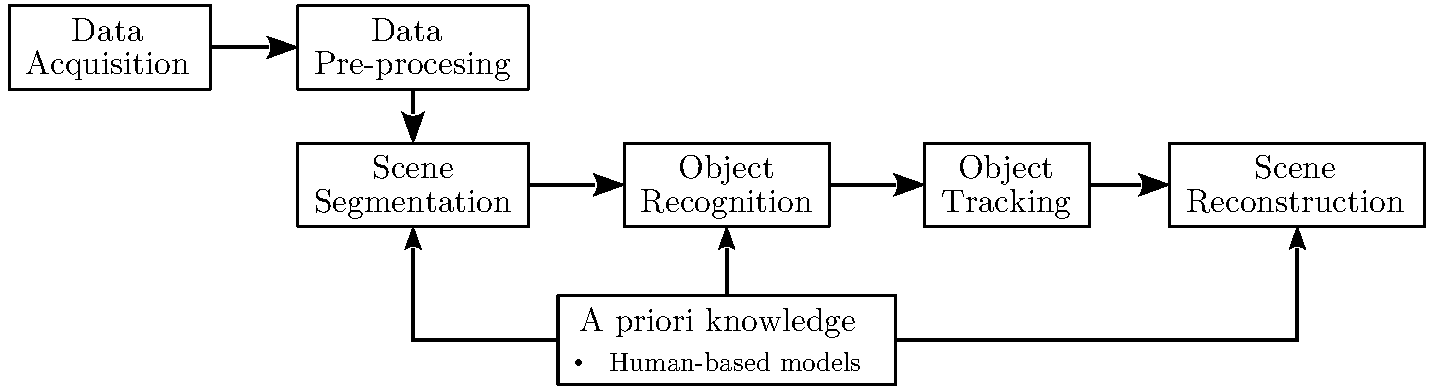
\includegraphics[width=\textwidth]{pipeline_scene_understanding_system}        
    \caption{Typical pipeline of a scene understanding system.}\label{fig:scene_understanding_systme_pipeline}
\end{figure}

Following the pipeline of Fig. \ref{fig:scene_understanding_systme_pipeline}, we can place the tasks of a scene understanding system into five general well-defined computer vision problems.

\begin{enumerate}[label=\roman*]
	\item \textbf{Image pre-processing}, whose objective is to remove the imperfections of an image generated by disturbances such as sensor noise or motion blur. Generally, we perform this task before passing it to a more complex algorithm. Image restoration and inpainting are some examples of this computer vision problem.
	
	\item \textbf{Image segmentation} is the process of partitioning an image into multiple (coherent) segments according to its features and properties. Depending on the application, we can formulate the image segmentation as the problem of classifying pixels with semantic labels (semantic segmentation), or partitioning of individual objects (instance segmentation), or both (panoptic segmentation).
	
	\item \textbf{Recognition} is a classic computer vision problem responsible for determining whether an image contains an object, characteristic, or exercise. Some variants of this problem are the classification, identification, and detection of objects from which many specialized tasks emerge. For example, content-based image search, pose estimation, optical character recognition, reading of 2-d codes, facial recognition, shape recognition, among others.
	
	\item \textbf{Motion analysis} is the problem that searches to estimate the speed of one or more points of interest within an image or 3-d scene by processing a sequence of images. Some examples of this task are egomotion, object tracking, pose estimation, and optical flow.
	
	\item \textbf{Scene reconstruction} is the problem related to the computation of a 3-d model from one or more images of a scene. This model is intended to be a description of the scene as close to reality as possible. 	
\end{enumerate}

These functionalities of computer vision and scene understanding systems are sought in the field of drones. UAVs (or drones) are flying engines that are increasingly present in our lives. We can find them in various sectors, such as the military, commercial or civil, where they can perform very specific tasks. However, in most cases, the development of such applications requires an expert pilot to control the aircraft. 

Commonly, the UAV control is achieved using conventional sensors, such as inertial sensors (IMUs) for orientation and GPS for position. The combination of information coming from these sensors in a flight computer allows the drones to remain stable in the air. However, IMUs present some drawbacks; for example, they suffer from bias error propagation due to the integral drift. On the other hand, the GPS signal is not always guaranteed; for example, the satellite signal may be low or unexisting in urban or indoor environments. A recurrent technique to enhance the drone's position accuracy implies the data fusion of pressure, ultrasonic, radars, and laser range-finders sensors \citep{Tomic.Schmid.ea:IRAM:2012}. The fusion of data can provide the advantages of each sensor. However, a significant limitation of these complex systems is flight time, a parameter mainly linked to the vehicle's total weight and the battery's capacity. Therefore, the use of multiple sensors onboard becomes expensive and impractical.

It is possible to extend the capabilities of a drone by integrating some visual sensor. Contrariwise to other sensors such as Lidars, visual sensors are passive, lightweight, and can acquire valuable information about the surrounding structures, including color and textures, and UAV's self-motion. The addition of visual sensors to perceive the environment has been a recurring strategy that has made these aerial robots more manipulable, safer, and even in some cases, autonomous \citep{He.Qiao.ea:CM:2018}, \citep{Kyrkou.Timotheou.ea:POT:2019}, \citep{Zhu.Wen.ea:arXiv:2020}.That means that the drone can perform a task without the need for human intervention. For this, the drone must be able to move without getting lost; moreover, it must interpret and understand the present scene so that it can be able to detect and avoid potential obstacles on its way. 

Today, one can use different visual sensors, such as monocular cameras \citep{Padhy.Xia.ea:TSC:2018}, stereo cameras \citep{Seitz.Curless.ea:CVPR:2006}, RGB-D cameras \citep{Huang.Bachrach.ea:RobR:2017}, fish-eye cameras \citep{Hrabar.Sukhatme:IROS:2004}, thermal cameras \citep{Gaszczak.Breckon.ea:IRCV:2011}, among others. This wide range of sensors offers more options and flexibility to deal with the problems mentioned above. The integration of such sensors in UAVs has allowed us to see the world from another perspective (literally), and the development of perceptual computer vision algorithms drives the technological improvement of these machines.

We know that today exist applications where vision algorithms have outstripped the capacity of human vision, so they have entirely replaced human personnel, for example, in industrial vision systems tasks, say, the inspection of production lines \citep{Malamas.Petrakis.ea:IVC:2003}. However, in other imaging areas, computer vision systems are only responsible for supplementing specific routines that require a considerable amount of time and experience from human experts. This discrepancy in the vision systems' performance is mainly related to the complexity of the task and the environment's conditions where the task is performed. In industrial vision systems, we can control the working conditions in most cases, while in areas such as robotics and unmanned aircraft (or UAV), with uncontrolled conditions and without large databases, computer vision algorithms bring a real challenge, even though the acquisition system is the same. 

\subsection*{Image Characteristics and Technical Locks in UAV Vision-based Applications}
%\markboth{Introduction}{Problem Statement}
%\section*{Computer Vision Problems in Drone Applications}
 
We can interpret the application and tasks made with drones as missions. Generally, such missions involve three central moments: take-off, navigation, and landing. The drone can perform such stages with conventional sensors; however, visual sensors provide valuable perceptual information about the environment.

Among the three moments that occur in drone missions, navigation and landing are the stages in which visual information (from onboard sensors) and computer vision algorithms most frequently intervene. In the landing stage, the needs and problems can be well-defined since it occurs at the end of the mission. Besides, we can control some conditions by adding pre-designed elements, such as landing targets or landing platforms, to facilitate the task. However, in the navigation stage, computer vision problems are mainly determined by the nature of drone applications.

Drone missions are generally carried out in complex scenes that change as the vehicle moves through space. For example, imagine all the scenarios that a delivery drone goes through during its mission: It can start its route in a commercial area, where the scenes mostly contain warehouses and big open spaces such as parking lots. Then, it could pass through rural areas, where the scenes can contain farmlands or wooded areas. Finally, when the drone reaches the delivery point within an urban zone, the environment may contain houses, trees, electricity, and telecommunications poles, among others. 

The mission through different environments generates considerable lighting changes and shadows, which results in overexposed and (or) dark images. Besides having no control over lighting conditions, we must also consider that the camera's position and orientation vary concerning the scene depending on the vehicle's height and orientation. Moreover, we must also consider the rolling shutter effect present in cameras using CMOS sensors. Therefore, the objects present in the images may have deformations because of the optic and the movement. Figure \ref{fig:img_drone_degradations} shows some images taken with a commercial drone in a natural setting. We can observe how the environment's lighting conditions and the nature of aerial applications introduce deformations to the images and objects present in the scene. 

Finally, we must not forget that we acquire the input images from an onboard camera, which is generally not stabilized; therefore, the images may be noisy or blurry. Such problems limit a computer vision algorithm to be globally efficient in all or most situations.


\begin{figure}[!ht]
    \centering
    \begin{subfigure}[b]{0.38\textwidth}
        \frame{\includegraphics[width=\textwidth]{Bebop_A}}
        \caption{Presence of shadows}
    \end{subfigure}
        ~ %add desired spacing between images, e. g. ~, \quad, \qquad, \hfill etc. 
      %(or a blank line to force the subfigure onto a new line)
    \begin{subfigure}[b]{0.38\textwidth}
        \frame{\includegraphics[width=\textwidth]{Bebop_B}}
        \caption{Saturations}
    \end{subfigure}
        ~ %add desired spacing between images, e. g. ~, \quad, \qquad, \hfill etc. 
      %(or a blank line to force the subfigure onto a new line)
    \begin{subfigure}[b]{0.38\textwidth}
        \frame{\includegraphics[width=\textwidth]{Bebop_C}}
        \caption{Change of scale}
    \end{subfigure} 
    \caption{Some examples of image degradations present in aerial imaging and UAV applications.}\label{fig:img_drone_degradations}
\end{figure}

In addition to the problems related to the complex scene conditions, we must consider that a drone is subject to sudden changes in the environment, such as wind gusts, which can affect its stability and modify the visual information given by the onboard sensors. In such cases, the vision algorithms for drone navigation must process the input information fast enough to provide answers and transform them into real-time decision actions.

Considering the conditions and problems of vision-based drone applications, we argue that a system for scene understanding is necessary for this kind of application. Moreover, scene understanding must use low-level information such as intensity, color, and texture in combination with perceptual tools to generate a robust image interpretation to the characteristic visual conditions of the aerial platforms. Among these classic computer vision problems, image segmentation is a crucial stage in the scene understanding pipeline. Image segmentation is a low-level task; however, it is critical for high-level applications such as classification, object tracking, reconstruction, and scene understanding. A robust segmentation to the changes and variants of complex environments allows the generalization of high-level tasks to new contexts and applications.

\section*{Image Segmentation State of the Art}
\markboth{Introduction}{Image Segmentation State of the Art}

Image segmentation has a long history in computer vision and is present in many applications in medicine, biology, robotics, and physics. Here, we present a brief review of the state-of-the-art segmentation methods taking into account the approach used and relationship with vision perception (a more detailed version of the state-of-the-art of segmentation methods appears in chapter \ref{ch:perceptual_object_boundaries_detection}, section \ref{sec:SoA_segmentation_methods}). For this purpose, we divide the image segmentation techniques into classical methods and Artificial Intelligence (AI) methods. 
%\cite{Khan:IJIG:2013}

\subsubsection*{Classical Image Segmentation Techniques} 
Classical image segmentation methods can be organized into two groups: those that identify similarities or those that identify discontinuities \citep{Zaitoun.Aqel:ICCMIT:2015}. The first kind of approach detects similar pixels in the image based on some specific threshold or criteria for split-merge and growing regions. The second category of methods tries to find the boundaries between dissimilar pixels in the image. A more specific classification according to the technique used divides segmentation methods into Threshold-based, edge-based, region-based, watershed-based, clustering-based, PDE-based, and Graph-based \citep{Zaitoun.Aqel:ICCMIT:2015}.

\textbf{Threshold-based} algorithms are one of the simplest image segmentation techniques. The threshold operation divides the image by comparing the intensity of the pixels to a specific threshold value\citep{Sezgin.Sankur:EI:2010}. This kind of method can only segment images into background and foreground based mainly on the intensity pixel information. This property is convenient when there is a significant contrast difference between the objects and the background. The major challenge of such approaches is the choice of the threshold value. The simplest option is to use a global threshold for the whole image; however, this option fails when the illumination in the image is uneven. Local thresholding methods solve this problem by proposing multiple thresholds \citep{Niblack:ImageProcc:1986}, \citep{Sauvola.Pietikainen:ICPR:2000}; however, the computation time can increase considerably. One of the most popular approaches in this category that automatically determine the threshold value is Otsu's method \citep{Otsu:SMC:1979}.

The \textbf{Edge-based} segmentation methods attempt to solve the image segmentation problem by detecting edges in an image according to the differences in texture, contrast, grey level, color, saturation, and other properties \citep{Saini.Arora:IJICT:2014}. Some of the more well-known methods in this category employ operators that use the first and second derivatives of the image to identify abrupt changes in the intensity of the image, for example, the Sobel \citep{Sobel.Feldman:SAIL:1990}, Roberts \citep{Roberts:Thesis:1963}, Gradient \citep{Maitre:Book:2003}, Prewitt \citep{Prewitt:PPP:1970}, and Laplacian \citep{Marr.Hildreth:PRS:1980} operators. On the other hand, one of the state-of-the-art reference work is the Probability-boundary (Pb) \citep{Malik.Belongie.ea:IJCV:2001},  which uses the intensity and color, and texture information to obtain the edges of the image. 

The \textbf{Region-based} segmentation methods partition the image into similar regions according to predefined criteria. Depending on the strategy used to arrive at the final segmentation, they can be organized into region growing and splitting and merging techniques \citep{Sezgin.Sankur:EI:2010}. Region growing techniques define a group of seed pixels from which regions start to grow \citep{Zucker:CGIP:1976, Adams.Bischof:TPAMI:1994}. Regions grow by appending to each seed pixel those neighboring pixels that have predefined properties similar to those of the seed pixels (e.g., intensity or color). Regions stop growing when they reach a particular predefined stop criterion (e.g., size or shape of the region).
Conversely, splitting and merging techniques do not require seed pixels. This technique successively divides the image into quadrants based on a homogeneity criterion, then similar regions are merged to form the final segmentation. This strategy includes the quad-tree data structure \citep{Horowitz.Pavlidis:ACM:1976}, which means a parent-child node relationship.
In practical applications, the region growing and splitting and merging algorithms are usually used in combination \citep{Ikonomatakis.Plataniotis.ea:ICDSP:1997}. This combination is more effective for the segmentation of complex scenes defined by some complex objects or the segmentation of certain natural scenes, such as image segmentation with insufficient prior knowledge.

The \textbf{Watershed-based} segmentation is a technique that utilizes image morphology and combines the characteristics of edge- and region-based methods described above. First, this method computes the gradient of an image. We can see this gradient as a map that reflects the topography of the image through the intensity values of the pixels. Then, segmenting an image is equivalent to flooding the topography from a group of seed pixels, where the edges of the image appear as the highest ridges where the flood water meets \citep{Meyer.Beucher:JVCIR:1990, Beucher.Meyer:Book:1993}. The watershed method is strictly linked to hierarchical segmentation methods \citep{Najman.Schmitt:PAMI:1996}. This feature of hierarchical dependence complexifies the efficient implementation in embedded processors. Many strategies introduce other definitions of the watershed transform to solve the complexity problem,  which simplifies and accelerates its computation \citep{Roerdink.Meijster:IOS:2000} , \citep{Dejnozkova.Dokladal:ICASSP:2003}, \citep{Chabardes.Dokladal.ea:ICIP:2016}.

Another alternative to obtain the segmentation of an image is by using clustering methods. The \textbf{clustering-based segmentation} methods are unsupervised techniques that classify the image pixels into clusters (disjoint groups) with similar features. The objective of pixel clustering is to maximize intra-class differences and minimize intra-class differences; that is, the pixels in each class should be as similar as possible, and those in the different groups should be as different as possible \citep{Steinley:BJMSP:2006}. The k-means technique is known as a hard-clustering technique since each pixel can belong only to one class. Fuzzy algorithms (soft-clustering) relax that condition, and each data point can belong to more than one cluster. This behavior is suitable in applications where there are no crisp boundaries between objects, such as tissue classification \citep{Caldairou.Passat.ea:PR:2011} and tumor detection \citep{Preetha.Suresh:CCT:2014}. Among the soft-clustering methods, fuzzy C-means clustering \citep{Dunn:JC:1973} is one of the most used.

\textbf{PDE-based} segmentation methods use Partial Differential Equations to model the image contours and obtain an image segmentation.  Active Contour Model (or Snakes) transform the segmentation problem into
PDE. Some famous methods of PDE used for image
segmentation are Snakes \citep{Kass.Witkin.ea:JCV:1988}, Level-Set \citep{Osher.Sethian:JCP:1988}, Fast Marching \citep{Forcadel.LeGuyader.ea:NA:2008}, and Mumford Shah method \citep{Mumford.Shah:CPAM:1989}. One of the main problems of these methods is the high computational time for the resolution of the PDE, which limits its use on embedded platforms. This limitation has been addressed in the implementation level through architectures that allow multi-core parallel calculation \citep{Dejnozkova.Dokladal:ICVIE:2003, Dejnozkova.Dokladal:ICASSP:2004}.

The last group of classical methods for image segmentation is \textbf{Graph-based}. These methods make use of graph theory to represent the image as a graph.  Typically, a pixel or a group of pixels are associated with nodes, and the edge weights define the affinity between neighboring pixels. Then, we can partition the graph according to a criterion designed to model good clusters. Each resulting partition of nodes is considered a segmented object in the image. Some popular algorithms in this category are normalized cuts \citep{JianboShi.Malik:PAMI:2000}, random walker \citep{Grady:PAMI:2006}, minimum cut \citep{Wu.Leahy:PAMI:1993}, isoperimetric partitioning \citep{Grady.Schwartz:PAMI:2006}, and minimum spanning tree \citep{Zahn:TC:1971}. Some of the segmentation methods can combine strategies. For example, spectral clustering \citep{Ng.Jordan.ea:NIPS:2001} uses the graph theory and the similarity of the graph edges to cluster the image pixels into coherent regions. On the other hand, \citep{Cousty.Bertrand.ea:PAMI:2009} define the watershed cuts cut on edge-weighted graphs using the Minimum Spanning Forest.

This group of approaches and techniques (known as classical, conventional, or traditional) can use structural, stochastic, or hybrid techniques to segment an image. Structural techniques require structural data from the image, such as distributions, histograms, pixel density, or color distribution. Stochastic techniques require information about the discrete values of the pixels. Machine learning methods, such as the clustering techniques, fall into this category. Finally, hybrid techniques may use structural information of image regions and the discrete values of the pixels of the whole image for the segmentation. The choice of the method to segment an image depends on the type of image and the type of segmentation that we seek to obtain (for example, over-segmentation or segmentation to pixel precision). Regardless of this, we consider it essential to consider the perceptual elements of the data to achieve a meaningful interpretation of the scene.

\subsubsection*{AI Image Segmentation Techniques} 
The \textbf{Artificial Neural Networks- (ANN) based} techniques (a.k.a. Deep Learning (DL) techniques) are probably the most widely used methods today because of their efficiency and accuracy. They are part of the supervised techniques, i.e., they require an annotated database for training, validation, and testing. In ANN-based methods, every neuron corresponds to the pixel of an image, which means the image is mapped to the neural network. Then, the image in the form of the neural network is trained using labeled data to find the connection between neurons (pixels). Lastly, the new images are segmented from the trained model. 

In recent years, neural network techniques (also known as deep learning (DL) techniques) have led to new models for image segmentation. We can classify these methods roughly according to the architecture they use. Convolutional Neural Networks  (CNNs) are among the most widely used and successful architectures in computer vision. This model, initially proposed by \cite{Fukushima:BC:1980}, is inspired by the model of the human visual cortex. Generally, CNNs contain convolution layers, non-linear layers (or activation functions) for feature mapping and pooling layers. Some of the best-known CNNs in the literature include LeNet \citep{Lecun.Bottou.ea::1998}, AlexNet \citep{Krizhevsky.Sutskever.ea:NIPS:2012}, VGGNet \citep{Simonyan.Zisserman:arXiv:2015} and ResNet \citep{He.Zhang.ea:ICVPR:2016}. 

Due to their characteristics, CNNs require dense layers and a large number of parameters, which makes them highly expensive. Fully Convolutional Networks (FCN) \citep{Long.Shelhamer.ea:CVPR:2015} solve this drawback by stacking several convolution Layers with similar padding to preserve the dimension and output a final segmentation map of the same size as the input image. Some of the best-known models are VGG16 and GoogleNet \citep{Szegedy.Liu.ea:arXiv:2014}.

Other deep learning backbones are the Encoder-Decoder and Auto-Encoder architectures. This type of model is known as two-stage networks. The first stage, encoding, compresses the input information into a space-latent representation, while the second stage, decoding, predicts an output from the representation. Some examples of networks that follow this architecture are DeConvNet \citep{Noh.Hong.ea:ICCV:2015}, SegNet \citep{Badrinarayanan.Kendall.ea:PAMI:2017}, U-Net \citep{Ronneberger.Fischer.ea:MICCAI:2015}, W-net \citep{Xia.Kulis:arXiv:2017}, Linknet \citep{Chaurasia.Culurciello:VCIP:2017}, among others.

Object detection and image segmentation are complementary tasks in computer vision. Similarly, exist architectures designed for object detection, such as Regional CNN (R-CNN), which have been successfully adapted for image segmentation. Some examples are the Faster R-CNN \citep{Ren.He.ea:PAMI:2017}, Mask R-CNN \citep{He.Gkioxari.ea:PAMI:2020} and Masklab \citep{Chen.Hermans.ea:CVPR:2018} architectures. The operation principle of these architectures is to extract the features of certain regions of interest to infer the class and the coordinates of the bounding box of the object.

A very recent family of architectures are those based on Generative Adversarial Networks (GANs) \citep{Goodfellow.Pouget-Abadie.ea:NIPS:2014}. This architecture consists of two networks, a generator, and a discriminator. The generator has the task of reproducing distributions similar to the real samples. On the other hand, the task of the discriminator is to distinguish the fakes samples from the real ones. GANs models include Convolutional-GANs \citep{Radford.Metz.ea:arXiv:2016}, Conditional-GANs \citep{Mirza.Osindero:arXiv:2014}, and Wasserstein-GANs \citep{Arjovsky.Chintala.ea:arXiv:2017}.

Other popular DL architectures for image segmentation include Feature Pyramidal Networks (FPN) \citep{Lin.Dollar.ea:CVPR:2017}, which takes a multi-scale approach, or hybrid ones that combine classical methods such as the Active Contour Model \citep{Kass.Witkin.ea:JCV:1988} and CNNs, or the watershed transform in the deep watershed architecture \citep{Bai.Urtasun:CVPR:2017}. 

The literature on methods based on DL architectures for image segmentation is vast. For a more detailed survey of the state of the art of ANN-based methods for image segmentation, please check \citep{Sultana.Sufian.ea:KBS:2020} and \citep{Minaee.Boykov.ea:PAMI:2021}.

%\citep{Kelm.Rao.ea:CAIP:2019}
AI-based image segmentation methods are experiencing popularity and growth that has benefited from advancements in computing power and the recent creation of publicly accessible annotated databases. However, its use in particular applications where there are not (yet) large enough annotated databases is complicated. Furthermore, despite the performance in challenging benchmarks, in many cases, the interpretability of the results of these methods remains open questions.

\subsubsection*{Vision-based UAV Navigation Related Works}
In the literature, we can find many works that deal with computer vision for drone navigation. The different approaches are strongly related and motivated by the application's aim and the conditions in which the task is developed. We can differentiate two main vision-based techniques for UAV navigation; 1) localization and mapping and 2) obstacle avoidance.

Simultaneous Localization and Mapping (SLAM) falls within the first group techniques, where drone navigation is a consistent result. This technique estimates the drone's local pose and builds a 3-d model of its surroundings employing visual sensors. Visual Odometry (VO) \citep{Scaramuzza.Fraundorfer:RAM:2011} is responsible for the robot motion estimation while the maps are built with occupancy grid algorithms \citep{Thrun.Bu:AI:1996}. According to the image information used to perform a SLAM, we can classify these approaches into feature-based methods, which extract a set of image features (e.g., lines, points) in a sequence of images, and direct-based methods, which make use of the image intensity information to estimate the structure and the motion of the robot \citep{Taketomi.Uchiyama.ea:TCVA:2017}. The importance of a correct segmentation of the image is that we can also create a depth chart of the scene from it and consequently achieve the visual odometry \citep{Drouyer:Thesis:2017, Drouyer.Beucher.ea:MMASP:2017}. 

The use of SLAM techniques for UAV navigation presents remarkable advantages. Feature-based methods can use various feature detectors, which typically count with an optimization stage to produce fast algorithms. Direct-based methods have the advantage of being robust to image degradations; they can lead better with images with texture and blurred zones; besides, the map produced is of an acceptable resolution. Interestingly, the strengths of the first group of methods are the weak points of the second and vice versa. A method that tries to gather the benefits of both approaches is the Semi-direct Visual Odometry \citep{Forster.Pizzoli.ea:ICRA:2014}; however, in general, the state-of-the-art SLAM methods is more mature in the autonomous vehicle environment \citep{Singandhupe.La:IRC:2019}.

There are approaches for drone navigation that, in parallel to SLAM, favor the avoidance of obstacles. This capability is essential for achieving free collision missions in both indoor and outdoor environments. A recurrent solution, as we early mentioned, is the multi-sensor data fusion. \cite{Gageik.Benz.ea:ACCESS:2015} present a platform using low-cost ultrasound and IR sensors; however, despite the obtained results, it utilizes several sensors to retrieve environment information, and yet, it does not get a perceptual representation of the scene due to the low resolution and perceptive capacity of the sensors. On the other hand, vision-based techniques for obstacle avoidance could detect obstacles and, in some cases, recognize and classify the object representing the obstacle \citep{Li.Ye.ea:IROS:2016}. 

We can classify the visual methods for avoidance of obstacles into two groups. The first, SLAM-based techniques, make use of the principles stated above. The 3-d reconstruction provides accurate and sophisticated maps and allows the air vehicle to travel with more information about the environment. In \citep{Moreno-Armendariz.Calvo:ICMEAE:2014}, takes this advantage to develop an obstacle avoidance approach for static and dynamic obstacles. The second group is the flow-based methods which historically, were inspired by the navigation of insects such as bees \citep{Srinivasan.Gregory:PTBS:1992} or flies \citep{Franceschini.Ruffier.ea:InTech:2009}. Many insects in the wild identify obstacles through the intensity of light. During the flight, their eyes produce an optical flow that provides accurate spatial information. Currently, there are also works inspired by the behavior of the human eye \citep{Al-Kaff.Meng.ea:IVS:2016}. The technique measures the object size from the idea that objects in the robot's vision field are more significant as the obstacle is close.

In general cases, obstacle avoidance techniques are strongly linked to the camera parameters and acquisition conditions. The algorithms are often fine-tuned. Given the condition, a drone operates in an environment without prior knowledge and under uncontrolled conditions. Hence some more general, unsupervised methods are needed.

Today, the most efficient algorithms are those based on Neural Network (NN) architectures and supervised learning techniques. Nevertheless, these techniques have remarkable disadvantages that question their usability and applicability in real-life drone missions \citep{Treboux.Genoud.ea:IWBIS:2018}. From a practical and even economic point of view, there is a limit to the number of applications in which we can use supervised methods given the fact that we need a lot of annotated data \citep{Xu.Wang.ea:CEA:2020}. The collection and the correct labeling of data representing a problem are valid only for a small number of applications.

The need for abundant information comes with high computational times required for model learning, ranging from a couple of hours to weeks. Of course, we can minimize this variable by increasing our machines' computing power; however, today, only those with large computing infrastructures can afford to train models with hundreds of billions of parameters.  

The above statement introduces the next disadvantage of deep neural network-based learning models: hyperparameters. We can roughly divide hyperparameters into two categories: 1) optimizer hyperparameters, which include the learning rate, the batch size, and the number of epochs, and 2) model-specific hyperparameters, which include the number of hidden layers, the first hidden layer, and the number of layers. Choosing the appropriate hyperparameters plays a crucial role in the success of neural network architectures because they control the learning algorithm's behavior, define the network structure, and define how the network is trained. Although there are methods to optimize their choice, generally, this task is a heuristic process, and their fine-tuning is a function of the specific application. It is possible to follow some rules based on experience, copy the same values from some other problem or make the setting by trial and error, though we cannot know the best value for a hyperparameter.

We can thus conclude that it is crucial to have the means to understand the scene, depending less on the parameters fixed in advance or the data sets prepared for a particular mission. In the following paragraphs, we present the contribution of this thesis to this issue.


%Nowadays, there is a wide variety of image segmentation techniques, some considered general-purpose and some designed for specific images.  On the other hand, \cite{Zaitoun.Aqel:ICCMIT:2015} propose a two-group classification: layer-based and block-based segmentation methods. Under these two taxonomies, we focus on classical or block-based segmentation methods. More specifically, we perform region-based segmentation and boundary-based segmentations.

\section*{Scope of the Thesis}
\markboth{Introduction}{Scope of the Thesis}
%First of all, this thesis work is motivated mainly by my profile and interests in robotics and control theory, specifically in air vehicles. 

The interaction between computer vision and applications made with unmanned aerial vehicles is extensive. This collaboration has generated new methodologies and approaches, both theoretical and practical, but has also given way to new research questions. 


Knowing the fundamental limitations of aerial robots and the complexity of drone applications, we explore computer vision theory to propose algorithms that improve and provide assistance in drone navigation tasks. In this sense, we are interested in studying the scene's perceptual information for their treatment and interpretation.

We focus primarily on the vision processing problems: object segmentation and recognition. We argue that two computer vision tasks are crucial for image understanding and have to be carefully treated in complex, uncontrolled environments. From this perspective, we focus on using low-level image features to extract perceptual information. 

Based on Fig. \ref{fig:scene_understanding_systme_pipeline} and considering the scope of the work in this thesis, we propose a new pipeline for scene understanding systems. In this new pipeline, the pre-processing of the image involves its perceptual decomposition, while the segmentation stage considers the perceptual elements of the image. The proposed pipeline for scene understanding is showed in Fig. \ref{fig:my_scene_understanding_systme_pipeline}. The peculiarity of this pipeline is that it eliminates the dependency on the a priori models, at least for the tasks of segmentation and image recognition (tasks that we study in this thesis). 

\begin{figure}[!ht]
    \centering
    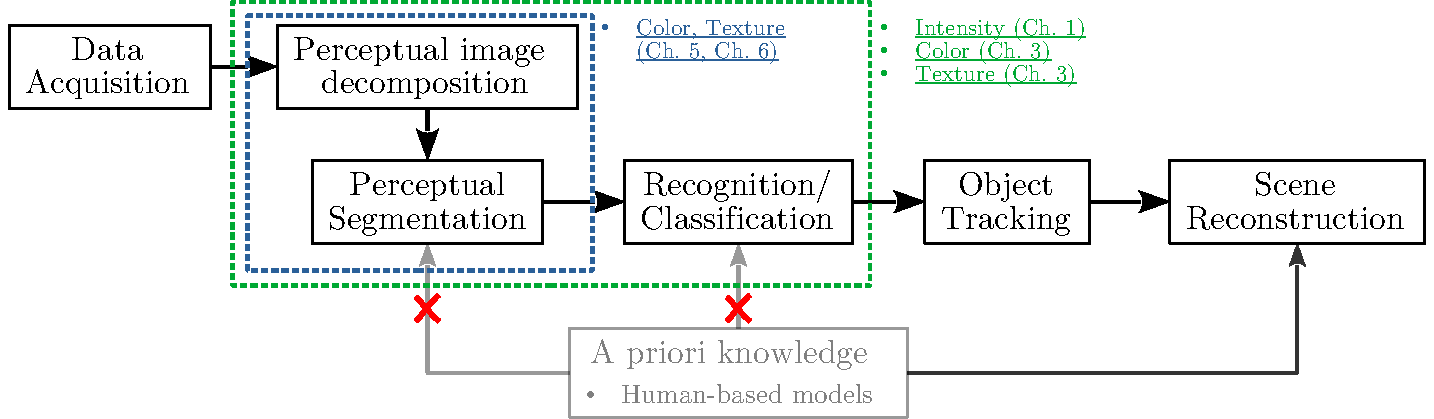
\includegraphics[width=\textwidth]{my_pipeline_scene_understanding_system}        
    \caption{Proposed pipeline of a scene understanding system.}\label{fig:my_scene_understanding_systme_pipeline}
\end{figure}

Throughout this work, we develop algorithms that are capable of handling a variety of real-world conditions. All these algorithms aim to segment the physical objects that we, as humans, define as perceptually interesting. For this purpose, we use intensity, color, and texture image information to extract low-level primitives, such as contours. In Fig. \ref{fig:my_scene_understanding_systme_pipeline}, we show the stages of scene understanding that we study in this thesis and the low-level primitives involved in the task: in green, the recognition and classification of objects use intensity, color, and texture, and in blue, the perceptual segmentation uses color, texture and the relationship between them. We use these primitives in conjunction with statistical and geometric tools from computer vision and signal theory, such as anomaly detector, optimal transport, and Gabor functions. Instead of using supervised methods, we focus on decomposing the image information from the point of view of signal theory and physics to use it later on non-supervised or mathematical morphology methods.
%So it is worth mentioning that the practical aspect linked to the implementation and the generation of solutions in real-time are not a priority. The developed algorithms provide solutions to the recognition and scene understanding problem's variants, such as the classification, identification, and detection of objects from a qualitative point of view, always looking for the application's physical meaning. 

Regarding the nature of the input data, we use only gray-level or color images as input information, favoring monocular cameras among the wide range of visual sensors reviewed previously. This choice allows replicating the algorithms with low-cost cameras that can be easily embedded in a drone.

%One last point about the focus of this work is about the type of computer vision techniques. The algorithms proposed in this thesis are based on traditional computer vision techniques, that is, non-deep learning techniques. This decision is consistent with drone applications' nature, where there are not necessarily rich enough annotated databases to apply the most sophisticated artificial intelligence models.

\section*{Contributions of the Thesis}\label{sec:objectives_of_the_thesis}
\markboth{Introduction}{Contributions of the Thesis}

%In this Ph.D. thesis, we aim to develop general computer vision algorithms considering the challenges and needs of UAV navigation. 

The primary objective of this Ph.D. thesis is to propose a new methodological framework for decomposing images before segmenting and detecting objects in the context of the scene understanding. The idea is to apply this methodological framework to assist in control and decision-making in drone navigation tasks. Therefore, the framework must be robust to image degradations existing in environments with uncontrolled conditions, in addition to being independent of the choice of specific parameters for its operation.

%During the thesis, we consider many specific drone tasks, such as:
%
%\begin{enumerate}[label=\roman*]
%	\item \textbf{Recognition} is a classic computer vision problem responsible for determining whether an image contains an object, characteristic, or exercise. Some variants of this problem are the classification, identification, and detection of objects from which many specialized tasks emerge. For example, content-based image search, pose estimation, optical character recognition, reading of 2-d codes, facial recognition, shape recognition, among others.
%	\item Environment awareness.
%	\item Detection and avoidance of obstacles.
%	\item Identification and following of targets.
%\end{enumerate}
%Given these tasks, the work focuses on the scene understanding problem. To deal with this problem, 
We extend the study of primary image information such as intensity, color, texture, and texture color and low-level image primitives such as contours. Therefore, some secondary objectives involve building a representation of the image in feature space using concepts from signal theory, geometry, and statistics, in addition to concepts from human perception. We seek to validate the proposed image representation using unsupervised approaches in real applications following traditional machine learning and segmentation algorithms.

Figure \ref{fig:general_diagram_framework} shows a general flowchart of the contributions of this thesis. The first stage of the flowchart shows low-level information and the methods we use to extract it; here, we work with intensity, color, texture, and the relationship between color and texture. The second stage of the diagram shows the different representations of the image obtained from the perceptual information contained in the primitives. Finally, the diagram's third section collects the different applications used to validate the image's feature spaces constructed in this thesis. Although the idea of a single framework itself is an ambitious goal, in this thesis, we present several algorithms that apply the proposed methodology with one or more features to solve different computer vision problems such as object detection and recognition, image retrieval systems, perceptual object boundaries detection, and image segmentation.

The interest of obtaining a representative space of the image information from low-level hand-made features lies in the possibility of using it in a semi-supervised pipeline. By injecting annotated information into the frame, it might make generalizations and obtain medium- or high-level features such as the importance of color and texture information to a human when segmenting an image. 

\begin{figure}[!ht]
    \centering
    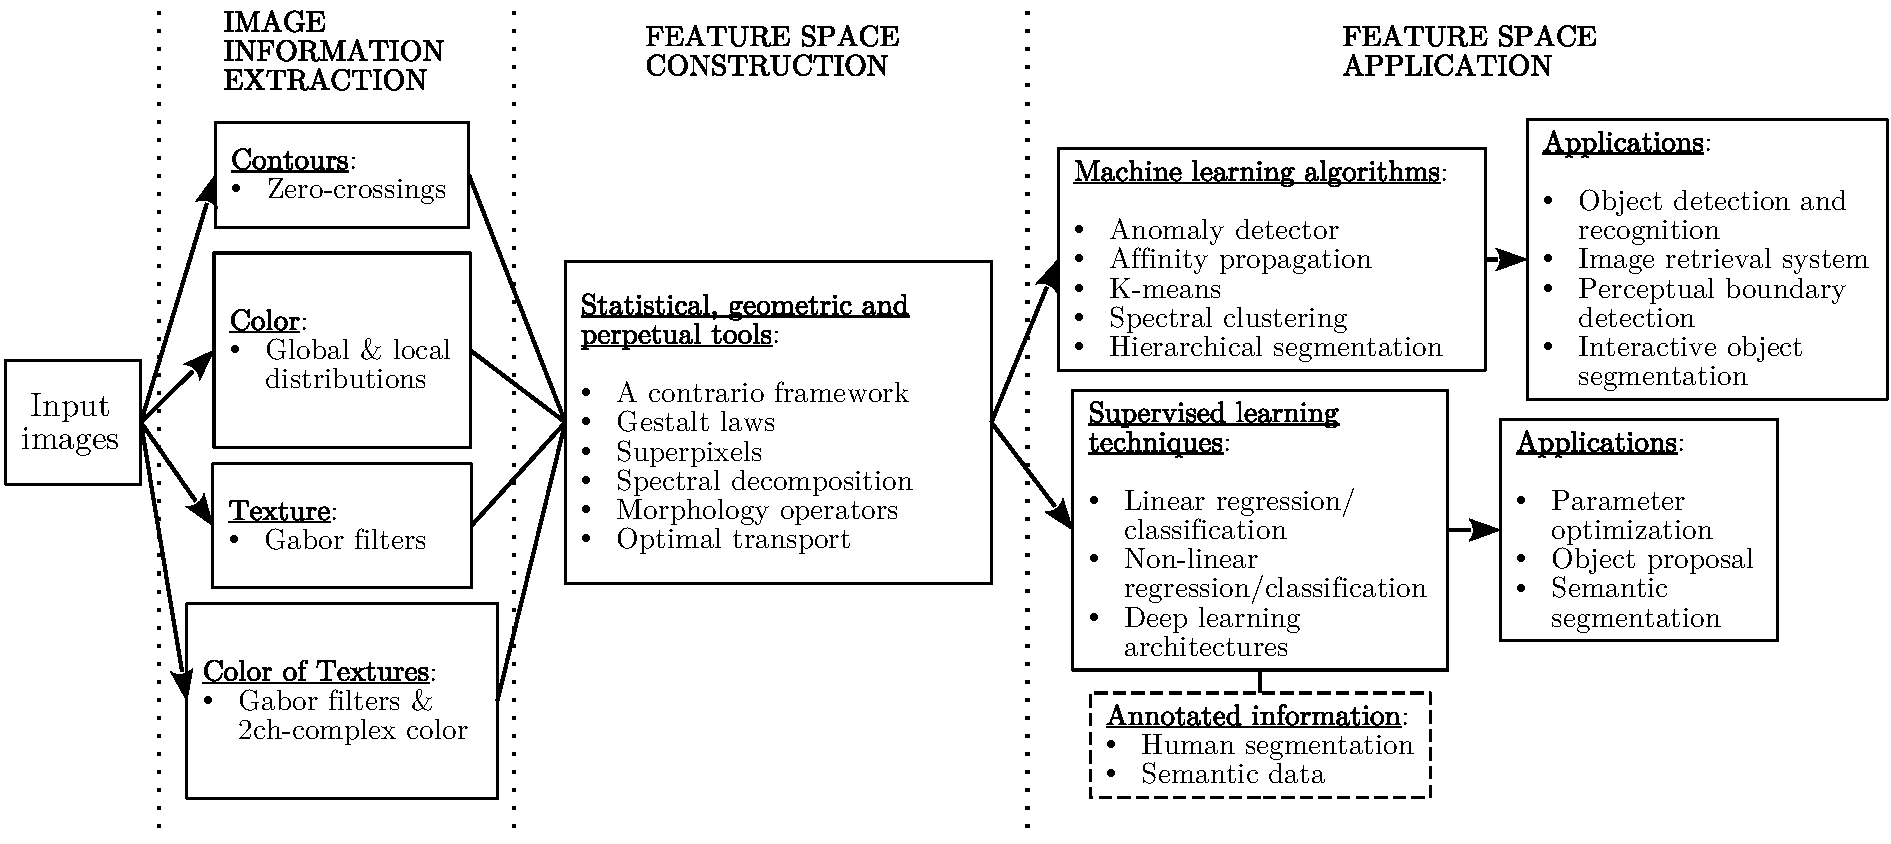
\includegraphics[width=\textwidth]{general_framework_diagram}        
    \caption{Flowchart of thesis contributions.}\label{fig:general_diagram_framework}
\end{figure}

Specifically, the contributions of this thesis include:

\begin{itemize}
	\item A novel non-parametric framework for fully unsupervised object detection robust to the image degradations present in complex, uncontrolled environments (chapter \ref{ch:landing_target_detection}).
	\item A qualitative and quantitative study between the most popular measures in the comparison of distributions (chapter \ref{ch:similarity_measures}). 
	\item An unsupervised image retrieval system based on global color/texture information (chapter \ref{ch:similarity_measures}).
	\item Extensive analysis of Gabor filters and their properties in the space-frequency domains (chapter \ref{ch:spectral_image_decomposition}).
	\item Generation of a feature space that includes the color and texture information of an image (chapter \ref{ch:complex_spectral_image_decomposition}).
	\item Unsupervised framework for natural image segmentation (chapter \ref{ch:perceptual_object_boundaries_detection}).
\end{itemize}

Finally, this thesis aims to show that traditional computer vision methods are (still) a reliable option to develop object detection and recognition for relatively complex tasks. We place this argument in the current context of computer vision, where there are hundreds of algorithms based on Neural Networks and Artificial Intelligence. Besides the NN and AI algorithms for image segmentation and object detection are highly performant, they lack a physical (and in many cases logical and argued) interpretation of its results. Furthermore, these algorithms are in trouble when it comes to image analysis of complex scenarios or applications where there is no database rich enough to do the learning process.


\section*{Organization of the Document}
\markboth{Introduction}{Organization of the Document}

To communicate our proposal and the objectives mentioned above in a clear and structured way, we present a thematic and chapter organization of the document. The thematic organization follows, to some extent, the complexity of the three low-level image information we used during this thesis: intensity, color, and texture. Then, we can identify three main parts in this thesis.

\begin{enumerate}
	\item The first part is dedicated to studying the intensity information of the image, in which we review in detail some of the classic methods for obtaining image contours. We use this information in conjunction with the \textit{a contrario} method and the Gestalt organizing laws to detect and identify landing targets. This part includes chapter \ref{ch:landing_target_detection}. 
	\item The second part main topic is studying the properties of color and texture of an image. We are interested in the global distribution of this information and the existing metrics to measure the similarity between the distributions; we apply and validate these concepts in two image retrieval systems. This part covers from chapter \ref{ch:color_texure_representations} to chapter \ref{ch:spectral_image_decomposition}.
	\item The third part extends the study of color and texture in images, exploding the local distribution of these primitives and studying the influence of color information on the generation of textures in an image. We propose a multi-spectral image decomposition helpful on the object segmentation tasks using classic clustering algorithms and for the generation of high-level texture features. Moreover, we propose a completely unsupervised framework for the detection of perceptual boundaries. We also explore different strategies to obtain the segmentation of natural images using the obtained perceptual boundaries. This part includes chapter \ref{ch:complex_spectral_image_decomposition} to chapter \ref{ch:perceptual_object_boundaries_detection}.
\end{enumerate}

The organization by chapters is structured as follows:

\begin{itemize}
	\item \textbf{Chapter \ref{ch:landing_target_detection}} addresses the bases of the Gestalt theory, including the grouping laws and the Helmholtz principle. We formalize these concepts of human perception mathematically and formulate a non-parametric algorithm that follows an unsupervised framework based on an image's contours. We use the developed framework in the autonomous drone landing problem, specifically detecting and identifying landing targets.  The chapter also presents a review and a quantitative comparison of different traditional methods for extracting image contours.
	
	\item \textbf{Chapter \ref{ch:color_texure_representations}} presents a detailed review of the different ways to represent the color and texture information in an image. The chapter contains a review of various color spaces and their main properties and an introduction to the different techniques for characterizing textures in the literature. Such information is of relevant importance in constructing the framework and the approaches to measure similarity between distributions.
	
	\item \textbf{Chapter \ref{ch:similarity_measures}} presents the analysis between different similarity measures between distributions, showing the advantages and disadvantages of each of them. In particular, we focus on the theory of optimal transport through the Earth Mover's Distance. We show the advantages of this metric over traditional similarity measures using an image retrieval system based on an image's global color and texture information.
	
	\item \textbf{Chapter \ref{ch:spectral_image_decomposition}} explores the physical and human perception aspects of Gabor's filters. We show the steps involved in designing an optimized and efficient Gabor family of filters. The proposed filter family models and captures the texture information through an energy-efficient decomposition of the image. Such spectral decomposition of the image deals with Heisenberg's uncertainty principle. The chapter presents the description of parameters that allow complete customization of the filter family according to the application.
	
	\item \textbf{Chapter \ref{ch:complex_spectral_image_decomposition}} brings an analysis of the texture information present in color images, showing the strong relationship between those two features. Using the spectral analysis of an image with the previously defined Gabor filters, we generate a feature space that simultaneously captures the color and texture information. We show the richness of such feature space by performing unsupervised image segmentation only using simple clustering techniques. Moreover, we show some novel high-level texture features resulting from the spectral image decomposition.
	
	\item \textbf{Chapter \ref{ch:perceptual_object_boundaries_detection}} introduces a framework for detecting perceptual boundaries of objects present in natural images. This framework brings together concepts addressed in this document, such as the spectral decomposition of images, the optimal transport as a true metric, and the relationship between color and texture information. Besides, using the hierarchical segmentation technique, we segment natural images in an unsupervised manner. We perform a quantitative and qualitative validation of our method using a known database.
	
%	\item \textbf{Chapter \ref{ch:general_conclusion}} contains the general conclusions of the thesis and addresses the different possible research lines as a continuation of this work.
	
\end{itemize}

